
%(BEGIN_QUESTION)
% Copyright 2012, Tony R. Kuphaldt, released under the Creative Commons Attribution License (v 1.0)
% This means you may do almost anything with this work of mine, so long as you give me proper credit

Sketch the necessary wiring to make this float-type level switch control a pump and a lamp in the following manner:

\begin{itemize}
\item{} High liquid level: pump on and lamp off
\item{} Low liquid level: pump off and lamp on
\end{itemize}

$$\includegraphics[width=15.5cm]{i01973x01.eps}$$

Hint: remember that the ``normal'' status of a switch is defined as the status of {\it minimum stimulus}: when the switch is exposed to the lowest possible degree of process stimulation (in this particular case, to the lowest possible level).


\underbar{file i01973}
%(END_QUESTION)





%(BEGIN_ANSWER)

This is just one possible solution:

$$\includegraphics[width=15.5cm]{i01973x02.eps}$$

%(END_ANSWER)





%(BEGIN_NOTES)


%INDEX% Pictorial circuit review (process switch circuit)

%(END_NOTES)


